\documentclass{beamer}
\usetheme{Madrid}
\usepackage{array}
\usepackage{tikz}
\usepackage{mathtools}
\title[CST 301 M2]{FORMAL LANGUAGES AND AUTOMATA THEORY}
\subtitle{Module 2}
\author{Rijin IK}
\institute[VJEC]{Assistant Professor\\Department of Computer Science and Engineering\\Vimal Jyothi Engineering College\\Chemperi}
\begin{document}
	\begin{frame}
		\titlepage
	\end{frame}
   \begin{frame}{Outline}
   \tableofcontents
   \end{frame}
\section{Course Outcomes}
\begin{frame}{Course Outcomes}
\textbf{After the completion of the course the student will be able to}
\begin{enumerate}
	\item Classify a given formal language into Regular, Context-Free, Context
	Sensitive, Recursive or Recursively Enumerable. [Cognitive knowledge
	level: Understand]
	\item Explain a formal representation of a given regular language as a finite state
	automaton, regular grammar, regular expression and Myhill-Nerode
	relation. [Cognitive knowledge level: Understand]
	\item Design a Pushdown Automaton and a Context-Free Grammar for a given
	context-free language. [Cognitive knowledge level : Apply]
	\item Design Turing machines as language acceptors or transducers. [Cognitive
	knowledge level: Apply]
	\item Explain the notion of decidability. [Cognitive knowledge level:
	Understand]
\end{enumerate}
\end{frame}
\section{Regular Expression (RE)}
\begin{frame}{Regular Expression (RE)}
	\textbf{Regular Expression (RE)}
	\begin{itemize}
		\item The languages accepted by finite automata are easily described by simple 
		expressions called regular expressions.
	\end{itemize} 
	\textbf{Formal Definition of Regular Expression (RE)}
		\begin{itemize}
		\item Let $\Sigma$ be an alphabet. The regular expressions over $\Sigma$ and the sets that they denote are defined recursively as follows.
		\begin{enumerate}
			\item $\phi$ is a regular expression and denotes the empty set. 
			\item $\epsilon$ is a regular expression and denotes the set $\{\epsilon\}$. 
			\item For each a in $\Sigma$, a is a regular expression and denotes the set $\{a\}$.
			\item If r and s are regular expressions denoting the languages R and S, 
			respectively, then
			$$(r + s), (rs),\  and\  (r^*)$$
			$$ \mbox{are regular expressions that denote the sets} $$
			$$ R \cup S, RS, and\  R^*, \mbox{respectively}.
$$ 
		\end{enumerate}
	\end{itemize}
\end{frame}
\begin{frame}{Regular Expression (RE)}
	\textbf{Q:}Write regular expressions for each of the following languages over 
	$\Sigma=\{0, 1\}$.

	\begin{enumerate}
		\item The set representing $\{00\}$. 
		\begin{itemize}
			\item $00 $
		\end{itemize}
		
		\item The set representing all strings of 0's and 1's.
		\begin{itemize}
			\item $(0+1)^*$
		\end{itemize}
		\item The set of all strings representing with at least two consecutive 0’s. 
	\begin{itemize}
		\item $	(0 + 1)^*00(0 + 1)^*$
	\end{itemize}
	\item The set of all strings ending in 011.
		\begin{itemize}
			\item $(0 + 1)^*011$
		\end{itemize}
	\item The set of all strings representing any number of 0's followed by any 
		number of 1’s followed by any number of 2's.
		\begin{itemize}
			\item $0^*1^*2^*$
		\end{itemize}
	\item The set of all strings starting with 011.
	\begin{itemize}
		\item $	011 (0 + 1)^*$
	\end{itemize}
	\end{enumerate}
\end{frame}
\begin{frame}{Regular Expression (RE)}
\textbf{Identity Rules Related to Regular Expressions}
\\ Given r, s and t are regular expressions, the following identities hold:
\begin{eqnarray*}
	\phi^* &=& \epsilon\\
	 \epsilon^* &=& \epsilon\\
	 r^+ &=& rr^* = r^*r\\
	 r^*r^* &=& r^*\\
	 (r^*)^* &=& r^*\\
	 r + s &=& s + r\\
	 (r + s) + t &=& r + (s + t)\\
	 (rs)t &=& r(st)\\
	 r(s + t) &=& rs + rt\\
	 (r + s)t &=& rt + st\\
	 (\epsilon + r)^* &=& r^*\\
\end{eqnarray*}
\end{frame}
\begin{frame}{Regular Expression (RE)}
	\small
	\textbf{Identity Rules Related to Regular Expressions cont..}
	\begin{eqnarray*}
		(r + s)^* &=& (r^*s^*)^* = (r^* + s^*)^* =(r+s^*)^*\\
		r + \phi &=& \phi + r = r \\
		r \epsilon &=& \epsilon r = r\\
		\phi L &=& L \phi = \phi\\
		r + r &=& r\\
		\epsilon + rr^* &=& \epsilon + r^*r = r^*
\\
	\end{eqnarray*}
\end{frame}
\subsection{Equivalence of Finite Automata and Regular Expressions}

\begin{frame}{Regular Expression (RE)}
	\begin{figure}
		\includegraphics[scale=.5]{img2/m1}
		\caption{Equivalence of Finite Automata and Regular Expressions}
	\end{figure}
\end{frame}
\begin{frame}{Equivalence of Finite Automata and Regular Expressions}
	\begin{itemize}
		\item The languages accepted by finite automata are precisely the 
		languages denoted by regular expressions. 
		\item For every regular expression there is an equivalent NFA with $\epsilon -
		transitions.$
		\item For every DFA there is a regular expression denoting its language.
	\end{itemize}
\end{frame}
\begin{frame}{Equivalence of Finite Automata and Regular Expressions}
	\begin{block}{Theorem}
		Let r be a regular expression then there exists an NFA with $\epsilon- transition$ that accept $L(r)$ 
	\end{block}
\proofname\\ 
\textbf{Zero operators}
	\begin{itemize}
		\item The expression r must be $\epsilon$, $\phi$, or a for some a in $\Sigma$. The NFA’s for zero operators are
		\begin{figure}
			\includegraphics[scale=.3]{img2/m2}
		\end{figure}
	\end{itemize}
\end{frame}
\begin{frame}{Equivalence of Finite Automata and Regular Expressions}

	\proofname \ cont.. 
	\textbf{One or more operators}
	\begin{itemize}
		\item Let r have i operators. There are three cases depending on the form of r.
	\end{itemize}
\textbf{Case 1: Union $(r = r1 + r2.)$}

\begin{itemize}
	\item There are NFA’s $M1 = (Q1, \Sigma1, \delta1, q1, \{f1\})$ and $M2=(Q2, \Sigma2, \delta2, q2, \{f2\})$ with $L(M1) = L(r1)$ and $L(M2) = L(r2)$.Construct $M = (Q1 \cup Q2 \cup \{q0, f0\}, \Sigma1 \cup \Sigma2, \delta, q0, \{f0\})$ where $\delta$ is defined by
	\begin{eqnarray*}
		\delta (q0, \epsilon) &=& \{q1,q2\}\\
		 \delta (q, a) &=& \delta1(q ,a)\  for\  q \ in\  Q1-\{f1\}\  and\  a \ in\  \Sigma1 \cup \{ \epsilon \}\\
		\delta (q, a) &=& \delta2(q ,a)\  for \ q\  in\  Q2-\{f2\} \ and\  a\  in \Sigma2 \cup \{ \epsilon \}\\
		 \delta (f1, \epsilon) &=& \delta1(f2, \epsilon) = \{ f0 \}\\
	\end{eqnarray*}
\end{itemize}
\end{frame}
\begin{frame}{Equivalence of Finite Automata and Regular Expressions}
	\proofname \ cont..\\ 
	$L(M) = L(M1) \cup L(M2)$
		\begin{figure}
		\includegraphics[scale=.3]{img2/m3}
		\caption{	$L(M) = L(M1) \cup L(M2)$}
	\end{figure}
\end{frame}
\begin{frame}{Equivalence of Finite Automata and Regular Expressions}
	\proofname \ cont..\\ 

	\textbf{Case 2: Concatenation $(r = r1 r2)$}
	\begin{itemize}
		\item Let M1 and M2 be as in Case 1 and construct $M = (Q1 \cup Q2, \Sigma1 \cup \sigma2, \delta,	q1, \{f2\})$
		\item where $\delta$ is defined by
	\begin{eqnarray*}
\delta (q,a) &=& \delta1(q ,a)\  for\  q \ in\  Q1-\{f1\} \ and\  a\  in\  \Sigma1 \cup \{\epsilon \} \\
\delta (f1, \epsilon) &=& \{q2\} \\
\delta (q, a) &=& \delta2(q ,a)\  for\  q \ in\  Q2 \ and\  a\  in\  \Sigma2 \cup \{ \epsilon\} \\
	\end{eqnarray*}
	\end{itemize}
$L(M) =\{xy|\ x \  is\   in\  L(M1)\  and\  y\  is\  in\  L(M2)\}\  and\  L(M)\  =\  L(M1)L(M2)$
	\begin{figure}
	\includegraphics[scale=.5]{img2/m4}
\end{figure}
\end{frame}
\begin{frame}{Equivalence of Finite Automata and Regular Expressions}
	\proofname \ cont..\\ 
	
	\textbf{Case 3: $Closure (r = r1^*)$}
	\begin{itemize}
		\item Let $M1 = (Q1, \Sigma1, \delta1, q1, \{f1\}) \ and\  L(M1) = r1$.
		\item Construct $M = (Q1 \cup \{q0,f0\}, \Sigma1 , \delta, q0, \{f0\})$, where $\delta$ is defined by
		\begin{eqnarray*}
			\delta (q0, \epsilon) &=& \delta (f1, \epsilon) = \{q1,f0\}\\
		    \delta (q, a) &=& \delta1(q ,a)\  for\  q in \ Q1-\{f1\}\  and\  a\  in\  \Sigma1 \cup \{ \epsilon \}\\
		\end{eqnarray*}
	\end{itemize}
	\begin{figure}
		\includegraphics[scale=.5]{img2/m5}
	\end{figure}
\end{frame}
\begin{frame}{Equivalence of Finite Automata and Regular Expressions}
\textbf{Q:}Construct an NFA for the regular expression $01^*+1$
\begin{itemize}
	\item Regular expression is of the form $r1 + r2$, where $r1 =01^*$ and $r2 = 1$.
	The automaton for r2 is 
	\begin{center}
		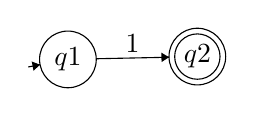
\begin{tikzpicture}[scale=0.12]
			\tikzstyle{every node}+=[inner sep=0pt]
			\draw [black] (18.2,-19.3) circle (3);
			\draw (18.2,-19.3) node {$q1$};
			\draw [black] (31.9,-19) circle (3);
			\draw (31.9,-19) node {$q2$};
			\draw [black] (31.9,-19) circle (2.4);
			\draw [black] (21.2,-19.23) -- (28.9,-19.07);
			\fill [black] (28.9,-19.07) -- (28.09,-18.58) -- (28.11,-19.58);
			\draw (25.04,-18.63) node [above] {$1$};
			\draw [black] (14,-20.1) -- (15.25,-19.86);
			\fill [black] (15.25,-19.86) -- (14.37,-19.52) -- (14.56,-20.5);
		\end{tikzpicture}
	\end{center}
\item Express r1 as r3 and r4, where r3=0 and $r4= 1^*$
The automaton for r3 is
\begin{center}
	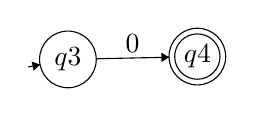
\begin{tikzpicture}[scale=0.12]
		\tikzstyle{every node}+=[inner sep=0pt]
		\draw [black] (18.2,-19.3) circle (3);
		\draw (18.2,-19.3) node {$q3$};
		\draw [black] (31.9,-19) circle (3);
		\draw (31.9,-19) node {$q4$};
		\draw [black] (31.9,-19) circle (2.4);
		\draw [black] (21.2,-19.23) -- (28.9,-19.07);
		\fill [black] (28.9,-19.07) -- (28.09,-18.58) -- (28.11,-19.58);
		\draw (25.04,-18.63) node [above] {$0$};
		\draw [black] (14,-20.1) -- (15.25,-19.86);
		\fill [black] (15.25,-19.86) -- (14.37,-19.52) -- (14.56,-20.5);
	\end{tikzpicture}
\end{center}
\item r4 is $r5^*$ where r5=1 The NFA for r5 is 
\begin{center}
	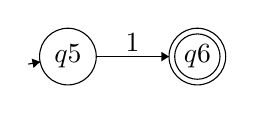
\begin{tikzpicture}[scale=0.12]
		\tikzstyle{every node}+=[inner sep=0pt]
		\draw [black] (18.2,-19.3) circle (3);
		\draw (18.2,-19.3) node {$q5$};
		\draw [black] (31.9,-19.3) circle (3);
		\draw (31.9,-19.3) node {$q6$};
		\draw [black] (31.9,-19.3) circle (2.4);
		\draw [black] (21.2,-19.3) -- (28.9,-19.3);
		\fill [black] (28.9,-19.3) -- (28.1,-18.8) -- (28.1,-19.8);
		\draw (25.05,-18.8) node [above] {$1$};
		\draw [black] (14,-20.1) -- (15.25,-19.86);
		\fill [black] (15.25,-19.86) -- (14.37,-19.52) -- (14.56,-20.5);
	\end{tikzpicture}
\end{center}
\end{itemize}
\end{frame}
\begin{frame}{Equivalence of Finite Automata and Regular Expressions}
	\begin{itemize}
		\item To construct an NFA for $r4 = r5^*$ use the construction of closure. The 
		resulting NFA for r4 is
		\begin{figure}
			\includegraphics[scale=.5]{img2/m6}
		\end{figure}
	\item Then, for $r1 = r3 r4$ use the construction of concatenation.
	\begin{figure}
		\includegraphics[scale=.3]{img2/m7}
	\end{figure}
	\end{itemize}
\end{frame}
\begin{frame}{Equivalence of Finite Automata and Regular Expressions}
	\begin{itemize}
		\item Finally, use the construction of union to find the NFA for $r = r1 + r2$
		\begin{figure}
			\includegraphics[scale=.3]{img2/m8}
		\end{figure}
	\end{itemize}
\end{frame}
\begin{frame}{Equivalence of Finite Automata and Regular Expressions}
	\textbf{Conversion of Finite Automata to Regular Expression}
	\begin{itemize}
		\item Any Regular Language can be represented by a Regular Expression.
	\end{itemize}
		\begin{figure}
		\includegraphics[scale=.5]{img2/m20}
	\end{figure}
\end{frame}
\begin{frame}{Equivalence of Finite Automata and Regular Expressions}
	Let $A$ be an NFA over an alphabet set $\Sigma$. Then:
	$$L_{p,q}=\{w\in\Sigma^* \big | \exists  a \ path\ from \ p \ to \ q\ with \ label \ as \ w\}$$ where p,q $\in$ Q
		\begin{figure}
		\includegraphics[scale=.5]{img2/m21}
	\end{figure}
\end{frame}

\begin{frame}{Equivalence of Finite Automata and Regular Expressions}
		Let $A$ be an NFA over an alphabet set $\Sigma$. Then the language of $A$
	$$L(A)=\bigcup_{f\in F} L_{s,f}$$
	where Q is the set of all states and F is the final state
		\begin{figure}
		\includegraphics[scale=.5]{img2/m22}
	\end{figure}
\end{frame}
\begin{frame}{Equivalence of Finite Automata and Regular Expressions}
		Let $A$ be an NFA over an alphabet set $\Sigma$. Then
	$$L_{p,q}^X=\{w \in \Sigma^* \big | \exists a \ path\ from \ p \ q\ with \ label \ as \ w \ passing \ through \ states \ in \ X\}$$
	where p, q $\in$ Q and X $\subseteq$ Q
		\begin{figure}
		\includegraphics[scale=.5]{img2/m23}
	\end{figure}
\end{frame}
\begin{frame}{Equivalence of Finite Automata and Regular Expressions}
	Let $A$ be an NFA over an alphabet set $\Sigma$. Then the language of $A$
	$$L(A)=\bigcup_{f\in F} L_{s,f}^Q$$
	$$R_{L(A)=\underset{f \in F}{+}R_{L_{s,f}^Q}}$$
	where Q is the set of all states and F is the final state
	\begin{figure}
		\includegraphics[scale=.5]{img2/m24}
	\end{figure}
\end{frame}
\begin{frame}{Equivalence of Finite Automata and Regular Expressions}
\textbf{Inductively defining RE from an NFA}
	\begin{figure}
	\includegraphics[scale=.5]{img2/m25}
\end{figure}
\end{frame}
\begin{frame}{Equivalence of Finite Automata and Regular Expressions}
\textbf{Kleen's Construction}
\begin{enumerate}
	\item Begin with $R_{L_{s,f}^Q}$ for all f $\in$ F
    \item Simplify using the terms with strictly small X's
	   $$R_{L_{p,q}^{x \cup \{r\}}}=R_{L_{p,q}^x }+R_{L_{p,r}^x }.(R_{L_{r,r}^x })^*.R_{L_{r,q}^x }$$
	   \item For the base terms, observe that:
\end{enumerate}
 \begin{equation*}
	R_{L_{p,q}^\phi }=\begin{cases}
		a, & \text{if $p\neq q$ and $\exists$ an edge for a from $p\  to\  q$}\\
		a+\epsilon, & \text{if $p=q$ and $\exists$ an edge for a from $p\  to\  q$}
	\end{cases}
\end{equation*}
 \end{frame}

\begin{frame}{Equivalence of Finite Automata and Regular Expressions}
	\textbf{Construction of regular expressions for the given finite Automata}
	\begin{block}{Arden’s Theorem}
		Let P and Q be two regular expressions over $\Sigma$,and if P does not contain 
		epsilon, then $R=Q+R$P has a unique solution $R=QP^*$
	\end{block}
\textbf{Procedure:}
\begin{itemize}
	\item Assume the given finite automata should not contain any epsilons.
	\begin{enumerate}
		\item Find the reachability for each and every state in given Finite 
		automata.
		\begin{itemize}
			\item \textbf{Reachability} of a state is the set of states whose edges enter into that state. 
		\end{itemize}
		\item For the initial state of finite automata ,add epsilon to the 
		reachability equation.
		\item Solve the equations by using Arden’s Theorem.
		\item Substitute the results of each state equation into the final state 
		equation,to get the regular expression for the given DFA.
		
	\end{enumerate}
\end{itemize}
\end{frame}
\begin{frame}{Equivalence of Finite Automata and Regular Expressions}
	\textbf{Q:}Construct regular expression for the given finite automaton.
\begin{center}
	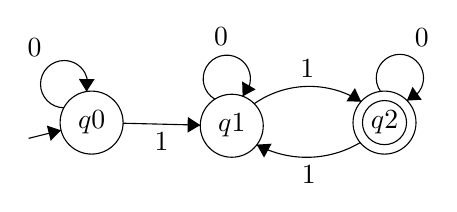
\begin{tikzpicture}[scale=0.2]
		\tikzstyle{every node}+=[inner sep=0pt]
		\draw [black] (13.2,-6.9) circle (2);
		\draw (13.2,-6.9) node {$q1$};
		\draw [black] (22.9,-6.7) circle (2);
		\draw (22.9,-6.7) node {$q2$};
		\draw [black] (22.9,-6.7) circle (1.4);
		\draw [black] (4.3,-6.7) circle (2);
		\draw (4.3,-6.7) node {$q0$};
		\draw [black] (14.622,-5.506) arc (125.05353:57.30885:6.102);
		\fill [black] (21.42,-5.37) -- (21.02,-4.51) -- (20.48,-5.35);
		\draw (17.99,-3.88) node [above] {$1$};
		\draw [black] (6.3,-6.74) -- (11.2,-6.86);
		\fill [black] (11.2,-6.86) -- (10.41,-6.34) -- (10.39,-7.34);
		\draw (8.74,-7.32) node [below] {$1$};
		\draw [black] (22.648,-4.724) arc (214.99737:-73.00263:1.5);
		\draw (25.27,-1.91) node [above] {$0$};
		\fill [black] (24.32,-5.3) -- (25.26,-5.25) -- (24.68,-4.43);
		\draw [black] (21.361,-7.966) arc (-59.17755:-118.46007:6.645);
		\fill [black] (14.79,-8.1) -- (15.25,-8.92) -- (15.73,-8.04);
		\draw (18.1,-9.42) node [below] {$1$};
		\draw [black] (12.136,-5.216) arc (240.00901:-47.99099:1.5);
		\draw (12.52,-1.84) node [above] {$0$};
		\fill [black] (13.89,-5.03) -- (14.72,-4.59) -- (13.86,-4.09);
		\draw [black] (2.544,-5.759) arc (269.53768:-18.46232:1.5);
		\draw (0.68,-2.54) node [above] {$0$};
		\fill [black] (3.98,-4.73) -- (4.49,-3.94) -- (3.49,-3.93);
		\draw [black] (0.3,-7.7) -- (2.36,-7.19);
		\fill [black] (2.36,-7.19) -- (1.46,-6.89) -- (1.7,-7.86);
	\end{tikzpicture}
\end{center}
\textbf{Solution:}
\begin{itemize}
	\item[1] Find the reachability for each and every state in given Finite 
	automata.

	\begin{eqnarray}
	q_0&=&q_0 0 \\
	q_1&=& q_0 1 + q_10 + q_2 1 \\
	q_2&=& q_1 1 + q_20 
	\end{eqnarray}
\end{itemize}
\end{frame}
\begin{frame}{Equivalence of Finite Automata and Regular Expressions}
	\textbf{Solution cont..}
	\begin{itemize}
		\item[2] For the initial state of finite automata, add epsilon to the 
		reachability equation.
		$q_0=q0_ 0 + \epsilon$
		\item[3] Solve the equations by using Arden’s Theorem.
		After applying arden’s theorem for equation 3

		\begin{eqnarray}
			q_2&=&q_1 10^*
		\end{eqnarray}
	Substitute equation 4 in equation 2
	\begin{eqnarray*}
	q_1&=& q_0 1 + q_10+q_1 10^*1
\end{eqnarray*}
	\begin{eqnarray}
q_1= q_0 1 + q_1(0+10^*1)
\end{eqnarray}
Apply arden’s theorem on equation 5
	\begin{eqnarray}
	q_1= q_01 (0+10^*1)^*
\end{eqnarray}
	\end{itemize}
\end{frame}
\begin{frame}{Equivalence of Finite Automata and Regular Expressions}
	\textbf{Solution cont..}
	Apply arden’s theorem on equation 1
	\begin{eqnarray*}
		q_0&=&q_0 0 + \epsilon
	\end{eqnarray*}
\begin{eqnarray}
	q_0&=& \epsilon 0^*
\end{eqnarray}
Substitute equation 7 in equation 6
\begin{eqnarray}
q_1&=& \epsilon 0^* 1 (0+10^*1)^*
\end{eqnarray}
\begin{itemize}
	\item[4] Substitute the results of each state equation into the final state 
	equation, to get the regular expression for the given DFA 
\end{itemize}
\begin{eqnarray}
	q_2&=& \epsilon 0^* 1 (0+10^*1)^* 10^*
\end{eqnarray}
Therefore, the regular expression for the given DFA is $0^* 1 (0+10^*1)^* 10^*$
\end{frame}
\section{Homomorphisms}
\begin{frame}{Homomorphisms}
	\textbf{Homomorphisms}
	\begin{itemize}
		\item A function mapping strings of one alphabet set to strings of other alphabet set.
	\end{itemize}
\textbf{Example}
\begin{itemize}
	\item Let $\Sigma = \{a,b,c\}$ and $\Gamma=\{0,1\}$ be two alphabet sets. Consider a homomorphism h defined as follows:\\
	$h(abab)=00010001$\ \ $h(bac)=010010$ \ \ $h(baba)=01000100$
	
\end{itemize}
	\begin{figure}
	\includegraphics[scale=.5]{img2/m27}
\end{figure}
 \end{frame}




\begin{frame}{Homomorphisms}
	\textbf{Homomorphisms-Definition}
	\begin{itemize}
		\item A Homomorphisms is a function h: $\Sigma^*\rightarrow \Gamma^*$ satisfying the following condition:
		$$\forall_{x,y} \in \Sigma^* \big | h(xy)= h(x)h(y)$$
	\end{itemize}
	\textbf{Example:}
	\begin{itemize}
		\item Let $\Sigma=\{a,b,c\}$ and $\Gamma=\{0,1\}$ be two alphabet sets. consider a homomorphism h defined as follows:
		\begin{itemize}
			\item $h(a)=00,h(b)=01,h(c)=10$ then ,
			\item $h(abcb)=h(a).h(b).h(c).h(b) = 00.01.10.01 = 00011001$
		\end{itemize}
	\item it follows from the property $h(xy)=h(x)h(y)$ of a homomorphism h that:
	$$\forall_{a_i} \in \Sigma \big | h(a_1a_2.....a_n)=h(a_1).h(a_2)...h(a_{n-1}).h(a_n)$$
	\end{itemize}
\end{frame}





\begin{frame}{Homomorphisms}
	\begin{block}{Theorem}
		If L is a regular language, and h is a 
		homomorphism on its alphabet, then $h(L)
	$ is also a regular 
		language
	\end{block}
\proofname \\
\begin{itemize}
	\item Let E be a regular expression for L.
	\item Apply h to each symbol in E.
	\item Language of resulting RE is h(L).
\end{itemize}
\end{frame}
\begin{frame}{Homomorphisms}
	\textbf{Q:}Using homomorphism on Regular Languages, Prove that the language $L=\{
		a^nb^nc^{2n} | n \geq 0\}$ is not regular. Given that the language $\{a^nb^n : n \geq 0 \}$ is not regular.\\
		\textbf{Solution: Proof by contradiction}
		\begin{itemize}
			\item Assume L is regular  That means that if h
			is a homomorphism and L
			is a regular language then h(L)
			is also regular.
			\item In This case you can take the homomorphism $h(a)=a
			, h(b)=b
			, h(c)=\epsilon$
			\item Which maps the language L to the language $h(L)=L'=\{a^nb^n:n\geq 0\}$  which you already know is not regular
			\item This contradiction shows that the language L is not regular.
		\end{itemize}
	
\end{frame}

\begin{frame}{Homomorphisms}
\textbf{Inverse Homomorphisms}
\begin{itemize}
	\item Let h:$\Sigma^* \rightarrow \Gamma^*$ be a homomorphism and $B\subseteq \Gamma^*$. Then its inverse homomorphism $h^{-1}:\Gamma^* \rightarrow \Sigma^*$ is defined as follows. $$h^{-1}(B) = \{x \in \Sigma^* |\  h(x)\in B\}$$
\end{itemize}
\textbf{Example:}
\begin{itemize}
	\item $h(a)=0,h(b)=1,h(c)=01$
	\item if we take $L=\{0011001\}$ then
	\item $h^{-1}(L)=\{aabbaab,aabbac,acbaab,acbac\}$
\end{itemize}
\end{frame}
\section{Pumping Lemma for regular languages }
\begin{frame}{Pumping Lemma for regular languages }
	\textbf{Pumping Lemma for Regular Sets}
	\begin{itemize}
		\item Pumping lemma, which is a powerful tool for proving certain 
		languages non-regular.

		\item It is also useful in the development of algorithms to answer certain 
		questions concerning finite automata, such as whether the language 
		accepted by a given FA is finite or infinite.
	\end{itemize}
\end{frame}
\begin{frame}{Pumping Lemma for regular languages }
	\textbf{Lemma}
	\begin{itemize}
		\item 	Let L be a regular set. Then there is a constant n such that if $x$ is any word 
		in L, and $|x| \ge n,$ we may write $x=uvw$ in such a way that $|uv| \leq n,\  v \geq 1,$ 
		and for all $i\ge 0$, $uv^iw$ is in L. 
		\item Furthermore, n is no greater than the number 
		of states of the smallest FA accepting L.
	\end{itemize}
\proofname \\
\begin{itemize}
	\item Since L regular there is a DFA $M$ which accept L.
	\item Let $n$ be  the number of states in $M$
	\item Consider an input of symbols $x=a_1a_2a_3…..a_m \  \in L$  where $m \geq n$
	\item Suppose we have a compassion sequence $ q_0,q_1,q_2,.....q_m $, representing the execution of automation M on input string $x$, and $q_m$ is an accepting state
	\item Here we have only $n$ distinct state , thus it is not possible for each state of M $(q_0 \ to \ q_m)$ to be distinct. So  at least two states should be equal. $(q_j=q_k \ say\  P \   where \ 0\leq j \leq k \leq n)$
\end{itemize}
\end{frame}
\begin{frame}{Pumping Lemma for regular languages }
	\proofname Cont..\\
	\begin{itemize}
		\item The path labeled $a_1a_2a_3…..a_m $ in the transition diagram of M is 
		\begin{figure}
			\includegraphics[scale=.5]{img2/m9}
		\end{figure}
		\item If $q_m$ is in f (i.e $a_1a_2a_3…..a_m $ is in $L(m)$) we can break the input x into three ie i.e $x=uvw$\\Where	
		\begin{eqnarray*}
			u &=& a_1a_2...a_j\\
			v &=& a_{j+1}a_{j+2}...a_k\\
			w &=& a_{k+1}a_{k+2}...a_m\\
		\end{eqnarray*}

	\end{itemize}
\end{frame}
\begin{frame}{Pumping Lemma for regular languages }
	\proofname Cont..\\
	\begin{itemize}
		\item 	So the transition function $\hat{\delta}(q_0,x) \in f$  becomes 
		\begin{itemize}
			\item $\hat{\delta}(q_0,u) = p$ 
			\item $\hat{\delta}(p,v) = p$ 
			\item $\hat{\delta}(p,w) = q_m$ 
			\item and also $\hat{\delta}(p,uw) = q_m$ 
		\end{itemize}
		Now it is clear for any $k \geq 0 ,\  uv^kw $ takes $q_0\  to\  q_m$  which is accepting. there for $xy^iz\ \in L$
	\end{itemize}
\end{frame}
\begin{frame}{Pumping Lemma for regular languages }
\textbf{Applications of Pumping Lemma}
\begin{itemize}
	\item Pumping Lemma is to be applied to show that certain languages are not regular.
\end{itemize}
\textbf{Method to prove that a language L is not regular}
\begin{enumerate}
	\item Assume that L is regular. Let n be the number of states in the corresponding finite automation
	\item Choose a string x such that $|x| \geq n$. Use pumping lemma to write $x = uvw$, with $|uv| \leq n$ and $|v| \geq 1$
	\item Find a suitable integer i such that $uv^iw \notin L.$ This contradicts our assumption. Hence L is not regular.
\end{enumerate}
The important part of proof is Step 3. There, we need to find i such that $uv^iw \notin L.$ 
\begin{itemize}
	\item In some cases, we prove $uv^iw \notin L.$ by considering $|uv^iw|$.
	\item In some cases, we may have to use the structure of strings in L.
\end{itemize}
\end{frame}

\begin{frame}{Pumping Lemma for regular languages }
	\textbf{Q:}Let  $L= \{0^k1^k:\  k \in N\}.$ Prove that L is not regular\\
	\textbf{Solution:}
.	\begin{itemize}
		\item By way of contradiction, suppose L is regular.
		\item Let n be an integer in the Pumping Lemma.
		\begin{eqnarray*}
			Let\  x &=& 0^n1^n\\
			&Then&  x \in L\ \  [definition \ of\  L] \\
			and\  |x| &=&2n \geq n.
		\end{eqnarray*}
	\end{itemize}
By Pumping Lemma, there are strings u, v, w such that
\begin{eqnarray*}
	&(i)& x = uvw,\\
	&(ii)& |v|\geq 1 ,\\
	&(iii)& |uv| \leq n,\\
	&(iv)& uv^iw \in L\  for\  all\  i \in N.
\\
\end{eqnarray*}
\end{frame}
\begin{frame}{Pumping Lemma for regular languages }
	\textbf{Solution Cont..}
	\\ Three cases are there  \\
	\textbf{Case 1:} v contain only 0's
	\begin{itemize}
		\item $v=0^k$  whewr  k$\geq$ 1
		\item there for $w=0^{n-k}0^k1^n$
		\begin{itemize}
			\item take i=0
			\begin{eqnarray*}
				uv^iw &=&uv^0w = uw\\
				&=&0^{n-k}0^n \notin L
			\end{eqnarray*}
		\end{itemize}
	\end{itemize}
	\textbf{Case 2:} v contain only 1's
	\begin{itemize}
		\item $v=1^k$  whewr  k$\geq$ 1
		\item there for $w=0^n1^k1^{n-k}$
		\begin{itemize}
			\item take i=0
			\begin{eqnarray*}
				uv^iw &=& uw\\
				&=&0^n1^{n-k} \notin L
			\end{eqnarray*}
		\end{itemize}
	\end{itemize}
\end{frame}
\begin{frame}{Pumping Lemma for regular languages }
	\textbf{Solution Cont..}\\
	\textbf{Case 3:} v contain both  0's and 1's
	\begin{itemize}
		\item $v=0^l1^m$  whewr  l\&m $\geq$ 1
		\item there for $w=0^{n-l}0^l1^m1^{n-m}$
		\begin{itemize}
			\item take i=0
			\begin{eqnarray*}
				uv^iw &=& uw\\
				&=&0^{n-l}1^{n-m} \ \ \  [\notin L \ or\ \in L\ depends \ on\  l\ \&\  m]
			\end{eqnarray*}
		\item take i=2
		\begin{eqnarray*}
			uv^iw &=& uv^2w\\
			&=&0^{n-l}(0^l1^m)^21^{n-m} \\
			&=&0^{n-l}0^l1^m0^l1^m1^{n-m}\\
			&=&0^n1^m0^l1^n \ \ \ \notin L
		\end{eqnarray*}
		\end{itemize}
	\end{itemize}
\end{frame}
\section{Ultimate periodicity}
\begin{frame}{Ultimate periodicity}
\textbf{Ultimate periodic Set}
\begin{itemize}
	\item A set which is periodic after a finite prefix is called an ultimately periodic set.
\end{itemize}
\textbf{Example}
\begin{itemize}
	\item Consider the following subset of $N_0$
\end{itemize}
	$$\{0,3,7,11,19,20,23,26,29,32,35,38,41,44,47,50,...\}$$
After the element 19, it is a periodic set with period 3. That is it contain every third element in $N_0$ from 20. 
\begin{block}{Formal Definition}
	A set U is called ultimately periodic if ther exists two natural numbers n$\geq$0 and $p>0$ such that $\forall m \geq n, m\in U\iff m + p\in U$
\end{block}
\begin{itemize}
	\item For an UP set U neither n nor p may be unique.
	\item Regular languages over singleton alphabet sets and UP sets are strongly related.
\end{itemize}
\end{frame}
\begin{frame}{Ultimate periodicity}
	\small
\begin{block}{Theorem}
Let A $\subseteq$ \{a\}*. Then A is regular if and only if the set $\{m |a^m \in A\}$, the 
set of lengths of strings in A, is ultimately periodic. 
\end{block}
\proofname :\\
\textbf{Part 1:} If A is regular, then the set $ \{m | a^m \in A\}$ is ultimately periodic.
\begin{itemize}
	\item Assume that A is regular, which means there exists a finite automaton that recognizes A. We want to show that the set $\{m | a^m \in A\}$ is ultimately periodic.
	\item Consider the lengths of strings in A. For each m, we want to determine whether $a^m$ is in A.
	\item We can simulate this using the finite automaton for A. Starting from the initial state, we can repeatedly apply transitions labeled 'a' for m times. If we end up in an accepting state after these m transitions, then $a^m$ is in A. Otherwise, it's not.
\end{itemize}
\end{frame}
\begin{frame}{Ultimate periodicity}

\begin{figure}
	\includegraphics[scale=.35]{img2/m10}
	\caption{Example}
\end{figure}
$lengths(L(A)) = \{2,5,8,11,14,17,20, . . . . .\}$
\begin{itemize}
	\item Now, observe that as we increase m, we are essentially repeating the same set of states in the finite automaton for A. 
	\item Since there are a finite number of states in the automaton, there must come a point where the states repeat. 
	\item This implies that the set of lengths $\{m | a^m \in A\}$ is ultimately periodic.
\end{itemize}
\end{frame}
\begin{frame}{Ultimate periodicity}
	\proofname cont..
	\begin{figure}
		\includegraphics[scale=.3]{img2/m11}
	%	\caption{$lengths(L(A)) = \{2\} \cup \{5, 11, 17, . . .\} \cup \{8, 14, 20, . . .\}$}
	\end{figure}
\small
\begin{itemize}
	\item Let p be the 
	length of the loop,
	\item  and let n be the length of the initial tail preceding the 
	first time we enter the loop.
	\item For all strings $a^m$ with $m \geq n$, the automaton 
	is in the loop part after scanning $a^m$ . Then $a^m$ is accepted iff $a^m +p$ is,
	\item since the automaton moves around the loop once under the last p a's of $a^m +p$ 
	\item Thus it is in the same state after scanning both strings.
	\item  Therefore, the set of lengths of accepted strings is ultimately periodic. 
\end{itemize}
\end{frame}
\begin{frame}{Ultimate periodicity}
	\proofname cont..\\
	\textbf{Part 2:} If the set $\{m | a^m \in A\}$ is ultimately periodic, then A is regular
	\begin{itemize}
		\item Given any ultimately periodic set U, 
		\item let p be the period and let n be the starting point of the periodic behavior. 
		\item Then one can build an automaton with a tail of length n and loop of length p accepting exactly the set of strings in $\{a\}^*$ whose lengths are in U.
	\end{itemize}
\end{frame}
\begin{frame}{Ultimate periodicity}
	\begin{block}{Corollary }
		Let L be any regular language over an arbitrary set $\Sigma$. Then the set $\{|x| \big| x \in L\}$ is ultimately	periodic.
	\end{block}
\proofname 
\begin{itemize}
	\item Take any regular language L.
	\item Define the homomorphism $h : \Sigma \rightarrow \{a\}\  by\  h(b) = a$ for all $b \in \Sigma$. 
	\item Then $h(x) = a^{|x|}$ . Since h preserves length, 
	\item we have that lengths $A =	lengths\  h(A)$. 
	\item But h(L) is a regular subset of $\{a\}^*$, since the regular 
		sets are closed under homomorphic image; 
	\item therefore, lengths h(L) is ultimately periodic.	
\end{itemize}
\end{frame}
\begin{frame}{Ultimate periodicity}
	\textbf{Application for ultimate periodicity}
	\begin{itemize}
		\item From the corollary we know that length set is ultimately periodic is a necessary condition for any regular language.
		\item Therefore, if we canprove that the length set of a given language L is not ultimately periodic, then we can conclude that L is not regular
		\item \textbf{Example:} 
		\begin{itemize}
			\item Let $L=\{a^{n!}\big| n\geq 0\}$  the length set :$\{1,2,6,24,120,...\}$ is  not ultimately periodic since the gap is monotonically increasing. Hence L is non regular
		\end{itemize}
	\item Length set is ultimatelyperiodic is not a sufficient condition for a language to be regular
	\item \textbf{Example:}
	\begin{itemize}
		\item  $L=\{a^nb^n\big| n\geq 0\}$  the length set :$\{0,2,4,6,8,10,12...\}$ is  ultimately periodic .But the language is not regular.
	\end{itemize}
	\end{itemize}
\end{frame}
\begin{frame}{Closure Properties of Regular Languages}
	\textbf{Let L and M be regular languages. Then the
		following languages are all regular:
}
\begin{enumerate}
	\item Union: $L \cup M$
	\item Intersection: $L \cap M$
	\item Complement: $\bar{N}$
	\item Difference: $L - M$
	\item Reversal: $L^R = {w^R : w \in L}$
	\item Kleene Closure: $L^*$
	\item Concatenation: $L.M$
	\item Homomorphism:
	\begin{itemize}
		\item $h(L) = \{h(w) : w \in L, h is a homom. \}$
	\end{itemize}
\item Inverse homomorphism:
\begin{itemize}
	\item $	h^{-1}(L) = \{w \big| h(w) \ is \ in \ L\}$
\end{itemize}
\end{enumerate}
\end{frame}
\begin{frame}{Closure Properties of Regular Languages}
	\textbf{Union: $L \cup M$}
	\begin{itemize}
		\item  For any regular L and M, $L\cup M$ is regular.
		\item The regular Languages are closed under Union
		\item Let $L=L(E)$ and	$M=	L(F)$. Then	$L\cup M =	L(E+F)$ by the definition of the $+$ operator.
	\end{itemize}
	\textbf{Intersection: $L \cap M$}
\begin{itemize}
	\item If L and M are regular, then	so is $L \cap M.$
	\item The regular Languages are closed under Intersection
\end{itemize}
\textbf{Complement: $\bar{N}$}
\begin{itemize}
	\item The complement of a language L (with respect to an alphabet $\Sigma$ such that $\Sigma*$ contains L) is $\Sigma^* – L$.
	\item Since $\Sigma*$ is surely regular, the complement of a regular language is always regular.
	\item The regular Languages are closed under Complement
\end{itemize}
\end{frame}
\begin{frame}{Closure Properties of Regular Languages}
	\textbf{Difference: $L - M$}
	\begin{itemize}
		\item If L and M are regular languages, then 
		so is $L – M$ = strings in L but not M.
		\item The regular Languages are closed under Difference: $L - M$
	\end{itemize}
	\textbf{Reversal: $L^R = {w^R : w \in L}$}
	\begin{itemize}
		\item If L is a regular language,
		then so is $L^R$.
		\item The regular Languages are closed under Reversal
	\end{itemize}
	\textbf{Kleene Closure: $L^*$}
	\begin{itemize}
		\item If L is a regular language,then so is $L^*$.
		\item The regular Languages are closed under  Kleene Closure
	\end{itemize}
\textbf{Concatenation: $L.M$}
\begin{itemize}
	\item If $L_1\ \& L_2 $ are two regular language,then so is $L_1L_2$ is also regular.
	\item The regular Languages are closed under  Concatenation
\end{itemize}
\end{frame}
\begin{frame}{Closure Properties of Regular Languages}
	\textbf{Homomorphism}
	\begin{itemize}
		\item If L is a regular language, and h is a 
		homomorphism on its alphabet, then $h(L)= \{h(w) \big|\  w\  is\  in\  L\}$ is also a regular 
		language.
		\item The regular Languages are closed under Homomorphism
	\end{itemize}
\textbf{Inverse Homomorphisms}
\begin{itemize}
	\item If h is a homomorphism from alphabet $\Sigma$ to alphabet	T, and L is a regular language over
	alphabet T, then $h^{-1}(L)$ is also a regular language
	\item The regular Languages are closed under Inverse Homomorphisms
\end{itemize}
\end{frame}
\section{Minimization of DFA}
\begin{frame}{Minimization of DFA}
		\begin{itemize}
			\item Minimization of DFA means reducing the number of states from given FA
			\item The minimization process consists of two stages
			\begin{enumerate}
				\item Get rid of inaccessible states
				\item Collapse ”equivalent” states
			\end{enumerate}
		\end{itemize}
	\textbf{Example}
		\begin{figure}
		\includegraphics[scale=.5]{img2/m12}
		%	\caption{$lengths(L(A)) = \{2\} \cup \{5, 11, 17, . . .\} \cup \{8, 14, 20, . . .\}$}
	\end{figure}
\end{frame}
\begin{frame}{Minimization of DFA}
	\begin{itemize}
		\item Minimization of DFA means reducing the number of states from given FA
		\item The minimization process consists of two stages
		\begin{enumerate}
			\item Get rid of inaccessible states
			\item Collapse ”equivalent” states
		\end{enumerate}
	\end{itemize}
	\textbf{Example}
	\begin{figure}
		\includegraphics[scale=.5]{img2/m12}
	\end{figure}
\end{frame}
\begin{frame}{Minimization of DFA-The Quotient Construction}
	One of the popular techniques for DFA state minimization is called the Quotient Construction.
	\begin{itemize}
		\item The Quotient Construction is based on the concept of equivalence classes.
		\item In this technique, the states of the original DFA are partitioned into different equivalence classes based on their behavior or language recognition capabilities.
		\item States within the same equivalence class are considered equivalent because they cannot be distinguished by any input sequence; they lead to the same final or non-final state.
	\end{itemize}
\end{frame}
\begin{frame}{Minimization of DFA-The Quotient Construction}
	\begin{itemize}
		\item The main idea is a process that takes a DFA and combines states of it in
		a step-by-step fashion, where each steps yields an equivalent automaton.
		\begin{itemize}
			\item We never combine a final state and a non-final state. Otherwise the
			language recognized by the automaton would change.

			\item If we merge states p and q, then we have to combine $\delta(p,a)$ and
			$\delta(q,a),$ for each $a \in \Sigma$
			\item Contrarily, if $\delta(p,a)\  and \ \delta(q,a)$ are not equivalent states, then p and q can not be equivalent.
		\end{itemize}
	\end{itemize}
\end{frame}
\begin{frame}{Minimization of DFA-The Quotient Construction}
	\textbf{DFA state equivalence}
	$$p \thickapprox q \xLeftrightarrow{def} iff \ \forall x\in \Sigma^*(\hat{\delta}(p, x) \in F \Leftrightarrow \hat{\delta} (q, x) \in F)$$
	where F is the set of final states of the automaton
	\begin{itemize}
		\item $\thickapprox$ is an equivalence relation, i.e., it is reflexive, symmetric, and
		transitive:
		\begin{eqnarray*}
			 p &\thickapprox& p\\
		 p &\thickapprox& q\implies q \thickapprox p\\
		 p &\thickapprox& q \land q \thickapprox r\implies p \thickapprox r
\\
		\end{eqnarray*}
	\end{itemize}
\end{frame}
\begin{frame}{Minimization of DFA-The Quotient Construction}
	\textbf{Quotient automaton}
	\begin{itemize}
		\item Let $M = (Q, \Sigma, \delta, q_0, F)$ be a DFA. The quotient automaton is $M / \thickapprox = (Q', \Sigma, \delta', q'_0 , F')$ where
		\begin{eqnarray*}
			Q'&\stackrel{\mathclap{\normalfont\mbox{def}}}{=}& \{ [p]\big| p\in Q \}\\
			\delta'([p],a)&\stackrel{\mathclap{\normalfont\mbox{def}}}{=}& [\delta(p,a)]\\
			q_0'&\stackrel{\mathclap{\normalfont\mbox{def}}}{=}& [q_0]\\
			F'&\stackrel{\mathclap{\normalfont\mbox{def}}}{=}& \{[p \big| p\in F]\}
		\end{eqnarray*}
	\end{itemize}
\end{frame}
\begin{frame}{Minimization of DFA-The Quotient Construction}
	\textbf{Quotient automaton}
	\begin{itemize}
		\item If M is a DFA that recognizes L, then$M/\thickapprox$  is a DFA that recognizes L. There is no DFA that both recognizes L and has fewer states than $M/\thickapprox$
	\end{itemize}
\end{frame}
\begin{frame}{Minimization of DFA-The Quotient Construction}
	\textbf{State Minimization Algorithm}
	\begin{enumerate}
		\item Write down a table of all pairs $\{p, q\}$, initially unmarked.
		\item Mark $\{p, q\}$ if $p \in F$ and $q \notin F$ or vice versa.
		\item Repeat the following until no more changes occur: 
		\begin{itemize}
			\item if there exists an unmarked pair $\{p, q\}$ such that $\{\delta(p, a), \delta(q, a)\}$ is marked for some $a \in \Sigma,$
			then mark $\{p, q\}$.
		\end{itemize}
		\item When done, $p \thickapprox q$ iff $\{p, q\}$ is not marked.
	\end{enumerate}


\end{frame}
\begin{frame}{Minimization of DFA-The Quotient Construction}
	Here are some things to note about this algorithm:
\begin{itemize}
	\item If $\{p, q\}$ is marked in step 2, then p and q are surely not equivalent: take
	$x = \epsilon$ in the definition of $\thickapprox$.
	\item We may have to look at the same pair $\{p, q\}$ many times in step 3, since
	any change in the table may suddenly allow $\{p, q\}$ to be marked. We stop
	only after we make an entire pass through the table with no new marks.
	\item The algorithm runs for only a finite number of steps, since there are only
	$\left( \begin{array}{c} n \\ 2 \end{array} \right)$
	possible marks that can be made, and we have to make at least one
	new mark in each pass to keep going.
	\item Step 4 is really a statement of the theorem that the algorithm correctly
	computes $ \thickapprox $.
\end{itemize}
\end{frame}
\begin{frame}{Minimization of DFA-The Quotient Construction}
\textbf{Example:}Minimize the following DFA
\begin{figure}
	\includegraphics[scale=.7]{img2/m13}
\end{figure}
\end{frame}
\begin{frame}{Minimization of DFA-The Quotient Construction}
	\textbf{Solution:}
\begin{itemize}
	\item We start by setting up our table. We will be able to restrict our attention
	to the lower left triangle, since equivalence is symmetric.
	\item Also, each box
	on the diagonal will be marked with $ \thickapprox $, since every state is equivalent to
	itself.
	\item  We also notice that state D is not reachable, so we will ignore it.

\end{itemize}
\begin{figure}
	\includegraphics[scale=.6]{img2/m14}
\end{figure}
\end{frame}
\begin{frame}{Minimization of DFA-The Quotient Construction}
	\textbf{Solution cont..}
	\begin{itemize}
		\item Now we split the states into final and non-final. 
		\item Thus, a box indexed by
		p, q will be labelled with an X if p is a final state and q is not, or vice versa.
	\end{itemize}
	\begin{figure}
		\includegraphics[scale=.5]{img2/m15}
	\end{figure}

\end{frame}
\begin{frame}{Minimization of DFA-The Quotient Construction}
	\textbf{Solution cont..}
	\begin{itemize}
		\item State C is inequivalent to all other states.
		\item Thus the row and column labelled by C get filled in with X0. (We will subscript each X with the step
		at which it is inserted into the table.)
		\item However, note that C, C is not filled
		in, since C$ \thickapprox $ C.
		\item Now we have the following pairs of states to consider:
		$$\{AB, AE, AF, AG, AH, BE, BF, BG, BH, EF, EG, EH, F G, F H, GH\}
$$
	\end{itemize}
\begin{itemize}
	\item Now we introduce some notation which compactly captures how the machine transitions from a pair of states to another pair of states. 
	$$p_1p_2 \xleftarrow{0} q_1q_2\xrightarrow{1}r_1r_2$$
\end{itemize}
\begin{itemize}
	\item means $q_1\xrightarrow{0} p_1$ and $q_2\xrightarrow{0}p_2$ and $q_1\xrightarrow{1}r_1$ and $q_2 \xrightarrow{1} r_2$
\end{itemize}
\end{frame}
\begin{frame}{Minimization of DFA-The Quotient Construction}
	\textbf{Solution cont..}
	\begin{itemize}
		\item If one of $p_1, p_2$,
		$r_1,\  or\  r_2$ are already marked in the table, then there is a way to distinguish
		$q_1 \ and\  q_2$: they transition to inequivalent states.
		\item Therefore $q_1 \not\approx  q2$ and the
		box labelled by $q_1q_2$ will become marked. For example, if we take the state
		pair AB, we have
		$$BG \xleftarrow{0} AB \xrightarrow{1} FC$$
	\end{itemize}
	\begin{itemize}
		\item and since FC is marked, AB becomes marked as well.
	\end{itemize}
	\begin{figure}
	\includegraphics[scale=.4]{img2/m16}
\end{figure}
\end{frame}
\begin{frame}{Minimization of DFA-The Quotient Construction}
	\small
	\begin{itemize}
		\item In a similar fashion, we examine the remaining unassigned pairs:
			\tiny
\begin{eqnarray*}
	BH \xleftarrow{0} AE &\xrightarrow{1}& F F. Unable to mark.\\
	BC \xleftarrow{0} AF &\xrightarrow{1}& F G. Mark, since \ BC\  is marked.\\
	BG \xleftarrow{0} AG &\xrightarrow{1}& F E. Unable to mark.\\
	BG \xleftarrow{0} AH &\xrightarrow{1}& F C. Mark, since \ FC\  is marked.\\
	GH \xleftarrow{0} BE &\xrightarrow{1}& CF. Mark, since \ CF\  is marked.\\
	GC \xleftarrow{0} BF &\xrightarrow{1}& CG. Mark, since \ CG\  is marked.\\
	GG \xleftarrow{0} BG &\xrightarrow{1}& CE. Mark, since \ CE\  is marked.\\
	GG \xleftarrow{0} BH &\xrightarrow{1}& CC. Unable to mark.\\
	HC \xleftarrow{0} EF &\xrightarrow{1}& F G. Mark, since \ CH\  is marked.\\
	HG \xleftarrow{0} EG &\xrightarrow{1}& F E. Unable to mark.\\
	HG \xleftarrow{0} EH &\xrightarrow{1}& F C. Mark, since \ CF\  is marked.\\
	CG \xleftarrow{0} FG &\xrightarrow{1}& GE. Mark, since \ CG\  is marked.\\
	CG \xleftarrow{0} FH &\xrightarrow{1}& GC. Mark, since \ CG\  is marked.\\
	GG \xleftarrow{0} GH &\xrightarrow{1}& EC. Mark, since \ EC\  is marked.
\\
\end{eqnarray*}
	\end{itemize}
\end{frame}
\begin{frame}{Minimization of DFA-The Quotient Construction}
\textbf{Solution cont..}
\begin{itemize}
	\item The resulting table is
\end{itemize}
	\begin{figure}
	\includegraphics[scale=.4]{img2/m17}
\end{figure}
Next round. The following pairs need to be considered:
$$\{AE, AG, BH, EG\}$$

\end{frame}
\begin{frame}{Minimization of DFA-The Quotient Construction}
	\textbf{Solution cont..}
\begin{itemize}
	\item The previously calculated transitions can be re-used;
	\item all that will have
	changed is whether the ‘transitioned-to’ states have been subsequently
	marked with an X1:
	\begin{itemize}
		\item AE: unable to mark
		\item	AG: mark because BG is now marked.
		\item	BH: unable to mark
		\item	EG: mark because HG is now marked
	\end{itemize}
\end{itemize}
\end{frame}
\begin{frame}{Minimization of DFA-The Quotient Construction}
	\textbf{Solution cont..}
	\begin{itemize}
		\item The resulting table is
	\end{itemize}
\begin{figure}
	\includegraphics[scale=.4]{img2/m18}
\end{figure}
\begin{itemize}
	\item Next round. The following pairs remain: $\{AE, BH\}$. 
	\item However, neither
	makes a transition to a marked pair, so the round adds no new markings
	to the table. 
	\item We are therefore done. The quotiented state set is
	$$\{\{A,E\},\{B,H\},\{F\},\{C\},\{G\}\}$$
\end{itemize}
\end{frame}

\begin{frame}{Minimization of DFA-The Quotient Construction}
	\textbf{Solution cont..}
	\begin{itemize}
		\item In other words, we have been able to merge states A and E, and B and H.
		The final automaton is given by the following diagram.
	\end{itemize}
	\begin{figure}
		\includegraphics[scale=.4]{img2/m19}
	\end{figure}
\end{frame}
\end{document}